\section{Deployment of a Kubernetes cluster, using two selected methods}
\textit{This is a practical chapter and it was written together with performing the empirical work and writing the source code. Main steps of Kubernetes cluster deployment will be described. Also, encountered problems will be listed and potential solutions will be presented.}
\\

\subsection{Experimental deployments using Kops}
\textit{In this subsection first experiments of deploying a Kubernetes cluster with Kops on AWS are described.}
\\

\subsubsection{Deployment without prerequisite steps done}

Although the aim of this work is to create a production Kubernetes cluster, it is always welcome, when there is a possibility to start working with a program easily. It is nice to have a simple working proof of concept (POC). Thus, it was decided to start with Kops without performing any prerequisite steps. The following commands were invoked:
\begin{lstlisting}[basicstyle=\tiny,caption={Commands used to create a cluster with kops, without prerequisite steps performed},captionpos=b,language=Bash,xleftmargin=1cm]
$ export KOPS_STATE_STORE=s3://dummy-k8s-kops-state-store
$ export NAME=dummy-k8s-kops.k8s.local
$ kops create cluster --state "s3://${K8S_EXP_KOPS_S3_BUCKET}" \
--master-zones=eu-west-1a --master-count=1 --master-size=t2.nano \
--zones=eu-west-1a --node-count=1 --node-size=t2.nano \
${NAME}
\end{lstlisting}


The command \textit{kops create cluster} instructs kops how to create a cluster. The flag \textit{--master-count=1} says that there will be one master node created, \textit{--master-size=t2.nano} sets the EC2 instance type and \textit{--master-zones=eu-west-1a} configures the AZs in which master nodes will be deployed. Similar flags are used to configure worker nodes. The \textit{--state} flag sets which S3 bucket to use.  \textbf{As expected and what is aligned with the Kops documentation\cite{online-kops-aws}, the above commands failed}, because the S3 bucket was not created. The command failed with the following output:
\begin{lstlisting}[basicstyle=\tiny,caption={Output of the commands used to create a cluster with Kops, without prerequisite steps performed},captionpos=b,language=Bash,xleftmargin=1cm]
error reading cluster configuration "dummy-k8s-kops.k8s.local":
error reading s3://dummy-k8s-kops-state-store/dummy-k8s-kops.k8s.local/config:
Could not retrieve location for AWS bucket dummy-k8s-kops-state-store
\end{lstlisting}

The Kops documentation\cite{online-kops-aws} informs that the following goals should be first accomplished, before deploying a Kubernetes cluster:
\begin{itemize}
\item AWS CLI tools should be installed
\item AWS credentials should be set
\item AWS IAM user and its permissions should be set
\item DNS should be configured
\item An S3 bucket should be created for storing a cluster state
\item AWS Region and Availability Zones should be chosen
\end{itemize}

Further in this chapter, after all the prerequisites will have been met, Kops will be used to create a production Kubernetes cluster.

\subsubsection{Deployment with prerequisite steps done - first working cluster}

First, all the prerequisites were done and they are described here. In order to make things simpler, an AWS user with administrator permissions was used. SSH keypair was already set. Then, it was decided to use the gossip-based DNS. Then, an S3 bucket was created to keep the Kops cluster configuration. Both versioning and server side encryption of the S3 bucket were enabled. Versioning was strongly recommended, because thanks to it, one may revert or recover a previous cluster state store. S3 bucket encryption is not required, but may be needed for compliance reasons\cite{online-kops-aws}. \textbf{Setting the S3 bucket} was done by the following commands:
\begin{lstlisting}[basicstyle=\tiny,caption={Commands used to set an AWS S3 bucket for Kops},captionpos=b,language=Bash,xleftmargin=1cm]
$ export K8S_EXP_REGION="eu-west-1"
$ export K8S_EXP_KOPS_S3_BUCKET="k8s-kops-for-masters-thesis.k8s.local"
$ export K8S_EXP_ENVIRONMENT="testing"
$ export K8S_EXP_CLUSTER_NAME="${K8S_EXP_ENVIRONMENT}.${K8S_EXP_KOPS_S3_BUCKET}"
$ aws s3api create-bucket --bucket ${K8S_EXP_KOPS_S3_BUCKET} --region ${K8S_EXP_REGION} \
--create-bucket-configuration LocationConstraint=${K8S_EXP_REGION}
$ aws s3api put-bucket-versioning --bucket ${K8S_EXP_KOPS_S3_BUCKET} \
--versioning-configuration Status=Enabled
$ aws s3api put-bucket-encryption --bucket ${K8S_EXP_KOPS_S3_BUCKET} \
--server-side-encryption-configuration '{"Rules":[{"ApplyServerSideEncryptionByDefault":{"SSEAlgorithm":"AES256"}}]}'
\end{lstlisting}

Then, \textbf{the command below was used to make Kops create the cluster configuration and put it in the S3 bucket}. The command is presented below together with its output:
\begin{lstlisting}[basicstyle=\tiny,caption={Command used to make Kops create the cluster configuration and put it in the S3 bucket},captionpos=b,language=Bash,xleftmargin=1cm]
$ kops create cluster --state "s3://${K8S_EXP_KOPS_S3_BUCKET}" \
--master-zones=eu-west-1a --master-count=1 --master-size=t2.nano \
--zones=eu-west-1a --node-count=1 --node-size=t2.nano ${K8S_EXP_CLUSTER_NAME}

error building tasks: error remapping manifest addons/kops-controller.addons.k8s.io/k8s-1.16.yaml: \
error parsing yaml: error converting YAML to JSON: yaml: line 56: did not find expected alphabetic or numeric character
\end{lstlisting}

Running this command resulted in \textbf{a not successful exit status (1)}. The reason for this was that the development environment had a non-numeric environment variable set. It was a password and the variable value contained asterisks (\textit{****}). After the variable was unset (with the bash command: \textit{unset}), the \textit{kops create cluster} succeeded. The output of this command presented the list of actions which Kops will perform on the AWS account, e.g. creating EBS volumes for Etcd, configuring IAM, creating keypairs for Kubernetes services, configuring network and setting EC2 instances. Details of the to-be-created resources were also provided, for example, the command output informed that the EC2 image will be: \textit{kope.io/k8s-1.16-debian-stretch-amd64-hvm-ebs-2020-01-17}. Apart from printing the output, Kops created a directory named the same as the cluster name (\textit{testing.k8s-kops-for-masters-thesis.k8s.local}) in the S3 bucket. Among the files automatically created by Kops, there is a configuration file named: \textit{config} and it contains the cluster settings. \textbf{The cluster configuration can be edited from command line} with the command presented below. Running this command starts a vim session.
\begin{lstlisting}[basicstyle=\tiny,caption={Command used to edit a Kubernetes cluster managed by Kops},captionpos=b,language=Bash,xleftmargin=1cm]
$ kops edit cluster ${K8S_EXP_CLUSTER_NAME} --state "s3://${K8S_EXP_KOPS_S3_BUCKET}"
\end{lstlisting}
After editing the configuration, \textbf{the cluster can be created or updated} (if it was created earlier) with the next command. This command deploys a cluster on AWS and prints a helpful output. Part of the output is also attached below:
\begin{lstlisting}[basicstyle=\tiny,caption={Command used to deploy a Kubernetes cluster with Kops},captionpos=b,language=Bash,xleftmargin=1cm]
$ kops update cluster ${K8S_EXP_CLUSTER_NAME} --state "s3://${K8S_EXP_KOPS_S3_BUCKET}" --yes

# some output lines omitted
Cluster is starting.  It should be ready in a few minutes.

Suggestions:
 * validate cluster: kops validate cluster
 * list nodes: kubectl get nodes --show-labels
 * ssh to the master: ssh -i ~/.ssh/id_rsa admin@api.testing.k8s-kops-for-masters-thesis.k8s.local
 * the admin user is specific to Debian. If not using Debian please use the appropriate user based on your OS.
 * read about installing addons at: https://github.com/kubernetes/kops/blob/master/docs/operations/addons.md.
\end{lstlisting}

Unfortunately, the commands listed as suggestions above did not work. They resulted in:
\begin{lstlisting}[basicstyle=\tiny,caption={Commands run in attempt to connect with a cluster created by Kops together with returned output},captionpos=b,language=Bash,xleftmargin=1cm]
$ kops validate cluster ${K8S_EXP_CLUSTER_NAME} --state "s3://${K8S_EXP_KOPS_S3_BUCKET}"
Validating cluster testing.k8s-kops-for-masters-thesis.k8s.local
unexpected error during validation: error listing nodes: \
Get https://api-testing-k8s-kops-for--l9puut-394396927.eu-west-1.elb.amazonaws.com/api/v1/nodes: EOF

$ ssh -i ~/.ssh/id_rsa admin@api.testing.k8s-kops-for-masters-thesis.k8s.local
ssh: Could not resolve hostname api.testing.k8s-kops-for-masters-thesis.k8s.local: \
Name does not resolve
\end{lstlisting}

It was expected that the latter command should fail, because \textit{api.testing.k8s-kops-for-masters-thesis.k8s.local} is not a public domain name and thus, it is not available from remote locations (such as this work author's computer). But the former command should have worked. In practice, there was no way to connect to the EC2 instances. Thus, as a solution - bigger EC2 instances were used: \textit{t2.micro} instead of \textit{t2.micro}. Using this particular instance type, \textit{t2.micro}, was observed in several online sources\cite{online-ha-k8s-blog}\cite{online-perfect-k8s-blog}\cite{online-kops-sa}. This time the command succeeded. It was possible to list the worker nodes with: \textit{kubectl get nodes}. It was doable thanks to kops creating an AWS Classic LoadBalancer. It exposed the following DNS A record that was publically reachable: \textit{api-testing-k8s-kops-for--l9puut-1371087518.eu-west-1.elb.amazonaws.com}.

It is also worth mentioning that the kubeconfig (\textit{~/.kube/config}), a Kubernetes configuration file needed to connect to a cluster, was generated automatically. Another thing to notice is that the command, which deploys a Kubernetes cluster, returned immediately, without waiting for the cluster to be ready. In the next deployments, some waiting mechanism must be applied, so that the cluster creation and verification can be automated. Below, there is a command used to request information about the cluster:
\begin{lstlisting}[basicstyle=\tiny,caption={Command used to request information about a running Kubernetes cluster},captionpos=b,language=Bash,xleftmargin=1cm]
$ kubectl cluster-info
Kubernetes master is running at https://api-testing-k8s-kops-for--l9puut-1371087518.eu-west-1.elb.amazonaws.com
KubeDNS is running at https://api-testing-k8s-kops-for--l9puut-1371087518.eu-west-1.elb.amazonaws.com/api/v1/namespaces/kube-system/services/kube-dns:dns/proxy

To further debug and diagnose cluster problems, use 'kubectl cluster-info dump'.
\end{lstlisting}

After the first cluster was successfully deployed, the following command was used in order export the cluster configuration into YAML file. It will be needed for production deployment.
\begin{lstlisting}[basicstyle=\tiny,caption={Command used to export a Kubernetes cluster configuration},captionpos=b,language=Bash,xleftmargin=1cm]
$ kops get -o yaml --name ${K8S_EXP_CLUSTER_NAME} --state "s3://${K8S_EXP_KOPS_S3_BUCKET}"
\end{lstlisting}

Then, \textbf{the cluster was deleted}. There were no problems with deleting the cluster. It took several minutes, but the following command succeeded and all the AWS resources (except for the manually created S3 bucket) were deleted:

\begin{lstlisting}[basicstyle=\tiny,caption={Command used to delete a Kubernetes cluster created with Kops},captionpos=b,language=Bash,xleftmargin=1cm]
$ kops delete cluster --name ${K8S_EXP_CLUSTER_NAME} --state "s3://${K8S_EXP_KOPS_S3_BUCKET}" --yes
\end{lstlisting}

The steps described in this section proved that it is possible to deploy a Kubernetes cluster on AWS with kops. It was a POC. The next cluster will attempt to satisfy the production deployment requirements.

%%%%%%%%%%%%%%%%%%%%%%%%%%%%%%%%%%%%%%%%%%%%%%%%%%%%%%%%%%%%%%%%%%%%%%%%%%%%%%%%
\subsection{Experimental deployments using eksctl}
\textit{In this subsection first experiments of deploying a Kubernetes cluster with eksctl on AWS are described.}
\\

In order to be consistent, the similar first experiment was performed using eksctl. It was decided to store the configuration locally in a YAML configuration file. The alternative was to set many command line flags. Below, \textbf{the configuration file and then the eksctl CLI command used to create a cluster are presented}:
\begin{lstlisting}[basicstyle=\tiny,caption={Commands used to create a cluster with eksctl, without prerequisite steps performed},captionpos=b,language=Bash,xleftmargin=1cm]
$ cat cluster.yaml
apiVersion: eksctl.io/v1alpha5
kind: ClusterConfig

metadata:
  name: cluster-eks
  region: eu-west-1

nodeGroups:
  - name: ng-1
    labels: { role: worker, cluster: cluster-eks }
    instanceType: t2.nano
    desiredCapacity: 1
    ssh:
      allow: true
$ eksctl create cluster -f cluster.yaml
\end{lstlisting}

This resulted in a successful creation of a cluster in "eu-west-1" AWS region with one worker node. Apart from that, the configuration file needed to access the remote cluster (remote, because deployed on AWS) was automatically created and written to: \textit{~/.kube/config} (same as done with kops). In order to \textbf{verify that the worker nodes were running}, the following command was run:
\begin{lstlisting}[basicstyle=\tiny,caption={Command used to list Kubernetes worker nodes to verify that one such node was running},captionpos=b,language=Bash,xleftmargin=1cm]
$ kubectl get nodes
NAME                                           STATUS   ROLES    AGE    VERSION
ip-192-168-176-90.eu-west-1.compute.internal   Ready    <none>   3m8s   v1.16.8
\end{lstlisting}

This experiment was successful. \textbf{It was easy to deploy a Kubernetes cluster using eksctl. No prerequisite steps were needed}. Besides, it was also easy to set up the YAML configuration file, basing on the eksctl documentation\cite{eksctl-creating-clusters}.


\textbf{The cluster was then deleted} with the following command:
\begin{lstlisting}[basicstyle=\tiny,caption={Command used to delete Kubernetes cluster with eksctl},captionpos=b,language=Bash,xleftmargin=1cm]
$ eksctl delete cluster -f cluster.yaml --wait
\end{lstlisting}

The \textit{--wait} CLI flag was applied. Without it, a delete operation would have been only requested but not waited for. In some cases it happens that the deletion fails, and, without this flag, the errors would not have been propagated back as the CLI command output. Then, one would be forced to delete the AWS resources manually\cite{eksctl-creating-clusters}.

%%%%%%%%%%%%%%%%%%%%%%%%%%%%%%%%%%%%%%%%%%%%%%%%%%%%%%%%%%%%%%%%%%%%%%%%%%%%%%%%

\subsection{Production deployment using Kops}
\textit{This section briefly presents all the steps performed that lead to a Kubernetes cluster deployment on the AWS cloud using Kops. Here an attempt was made to satisfy all the production environment requirements selected in the chapter: \ref{prep-prod}.}
\\

\subsubsection{Generating the YAML configuration file}
In contrast to the experimental deployment, here the cluster was configured with a YAML file. What is more, the YAML file was a Go (golang) template file\cite{online-kops-ct}, thanks to what it was easy to set the environment. (Two environments were supported: testing and production). Creating the YAML file is not recommended to be done by hand. Rather, one should first run \textit{kops create cluster} command (which creates a cluster configureation in a S3 bucket state store) and then export the configuration from the state store with: \textit{kops get -o yaml}. There are plans to change it. Using YAML instead of CLI has another advantage: more options can be set\cite{online-kops-manifest} and addons can be deployed\cite{online-kops-addons}.

First, a S3 bucket was created in the same way as in the experimental deployment. Then, the cluster kops YAML configuration file was generated with:
\begin{lstlisting}[basicstyle=\tiny,caption={Commands used to generate a cluster configuration with kops},captionpos=b,language=Bash,xleftmargin=1cm]
$ my_ip=$(curl https://ipinfo.io/ip 2>/dev/null)
kops create cluster --state="s3://${K8S_EXP_KOPS_S3_BUCKET}" \
--kubernetes-version=1.16.9 \
--master-zones="eu-west-1a,eu-west-1b,eu-west-1c" --master-count=3 --master-size=t2.micro \
--zones=eu-west-1a --node-count=1 --node-size=t2.micro \
--ssh-access=${my_ip}/32 \
${K8S_EXP_CLUSTER_NAME}
\end{lstlisting}

The following options were set:
\begin{itemize}
\item \textit{$--state="s3://\${K8S\_EXP\_KOPS\_S3\_BUCKET}"$} to set a S3 bucket name
\item \textit{--kubernetes-version=1.16.9} to choose a particular Kubernetes version
\item \textit{--master-zones="eu-west-1a,eu-west-1b,eu-west-1c"} to choose AZs for master instances (to ensure HA)
\item \textit{--master-count=3} to deploy 3 master nodes
\item \textit{--master-size=t2.micro} to choose EC2 instance type for master nodes
\item \textit{--zones="eu-west-1a"} to choose AZs for node instances
\item \textit{--node-count=1} to deploy 1 worker node
\item \textit{--node-size=t2.micro} to choose EC2 instance type for worker nodes
\item \textit{--ssh-access=\${my\_ip}/32} to apply more security
\end{itemize}

Then, the configuration was exported to local filesystem, as a configuration template:
\begin{lstlisting}[basicstyle=\tiny,caption={Command used export kops configuration from S3 to a local file},captionpos=b,language=Bash,xleftmargin=1cm]
$ kops get -o yaml --name ${K8S_EXP_CLUSTER_NAME} --state "s3://${K8S_EXP_KOPS_S3_BUCKET}" > cluster.tmpl.yaml
\end{lstlisting}

Afterwards, that configuration template file was edited, so that \textit{kubernetesApiAccess} and \textit{sshAccess} were set in order to ensure more security - only one IP was allowed to communicate with the Kubernetes cluster. Then, in that file, all the occurrences of the word: "testing" were replaced with: "{{.environment}}". Thanks to that, it is now possible to decide on the environment at the moment of cluster deployment. As the third edit done to that file: \textit{cloudLabels} were specified, so that it is easier to identify which AWS resources belong to this Kubernetes deployment\cite{online-kops-labels}. The next edit was needed to add IAM permissions, so that Kubernetes logs may go to AWS CloudWatch. The following code was added to the \textit{cluster.tmpl.yaml} file:
\begin{lstlisting}[basicstyle=\tiny,caption={TODO},captionpos=b,language=Bash,xleftmargin=1cm]
additionalPolicies:
  node: |
      [
        {
          "Effect": "Allow",
          "Action": ["logs:CreateLogGroup", "logs:CreateLogStream", "logs:PutLogEvents", "logs:DescribeLogGroups", "logs:DescribeLogStreams"],
          "Resource": ["*"]
        }
      ]
  master: |
      [
        {
          "Effect": "Allow",
          "Action": ["logs:CreateLogGroup", "logs:CreateLogStream", "logs:PutLogEvents", "logs:DescribeLogGroups", "logs:DescribeLogStreams"],
          "Resource": ["*"]
        }
      ]
\end{lstlisting}

Then, the template configuration file was compiled into two configuration files, one for each environment:
\begin{lstlisting}[basicstyle=\tiny,caption={TODO},captionpos=b,language=Bash,xleftmargin=1cm]
$ kops toolbox template --name ${K8S_EXP_CLUSTER_NAME} --set environment=testing --template cluster.tmpl.yaml --format-yaml > cluster-testing.yaml
$ kops toolbox template --name ${K8S_EXP_CLUSTER_NAME} --set environment=production --template cluster.tmpl.yaml --format-yaml > cluster-production.yaml
\end{lstlisting}
Most of this work is implemented in the Bash script and can be run as:
\begin{lstlisting}[basicstyle=\tiny,caption={TODO},captionpos=b,language=Bash,xleftmargin=1cm]
$ ./tasks _gen_config
# then perform the twinkering described above (set IAM permissions, labels and security settings)
$ ./tasks _up_remote_config
\end{lstlisting}

In result, two YAML configuration files were created: for testing and for production environments. The procedure was semi-automated, it should be easy to change the YAML file.

\subsubsection{Creating the cluster}
\label{kops-creating-the-cluster}
All the work described in this section, needed to deploy a Kubernetes cluster is fully automated. In the future it may be used in a CI pipeline. This step can be executed with one command:
\begin{lstlisting}[basicstyle=\tiny,caption={TODO},captionpos=b,language=Bash,xleftmargin=1cm]
$ ./kops/tasks _create
\end{lstlisting}

The rest of this section describes what this one command provides. This command provides several things. First, it updates the cluster configuration in S3 bucket, based on the local YAML configuration file. Then, it creates AWS resources needed for Kubernetes cluster (EC2 instances, VPC, etc.). Then, it was decided that this command should return only after the Kubernetes cluster is ready. Thus, a simple Bash loop was implemented, which verifies if a cluster is ready, every 1 second. The code for these commands is presented below:
\begin{lstlisting}[basicstyle=\tiny,caption={TODO},captionpos=b,language=Bash,xleftmargin=1cm]
kops replace -f cluster-${K8S_EXP_ENVIRONMENT}.yaml --name ${K8S_EXP_CLUSTER_NAME} --state "s3://${K8S_EXP_KOPS_S3_BUCKET}"
kops update cluster ${K8S_EXP_CLUSTER_NAME} --state "s3://${K8S_EXP_KOPS_S3_BUCKET}" --yes
# wait for the deployment to finish
while [ 1 ]; do
  kops validate cluster ${K8S_EXP_CLUSTER_NAME} --state "s3://${K8S_EXP_KOPS_S3_BUCKET}" && break || sleep 30
done;
\end{lstlisting}

So far, all the necessary work was performed in order to have a working cluster. The next thing is to deploy logging. The following code was needed to attain this goal:
\begin{lstlisting}[basicstyle=\tiny,caption={TODO},captionpos=b,language=Bash,xleftmargin=1cm]
$ aws logs create-log-group --log-group-name k8s-kops-${K8S_EXP_ENVIRONMENT}
$ helm install "kube2iam" --namespace="default" --wait --atomic --set rbac.create=true stable/kube2iam
$ helm repo add incubator https://kubernetes-charts-incubator.storage.googleapis.com
$ helm install "fluentd-cloudwatch" --namespace="default" --wait --atomic --set awsRegion=${K8S_EXP_REGION},rbac.create=true,logGroupName=k8s-kops-${K8S_EXP_ENVIRONMENT} incubator/fluentd-cloudwatch
\end{lstlisting}

An AWS CloudWatch LogGroup was created first. Then, two Helm charts were deployed. The kube2iam chart handles the permissions of Kubernetes pods and the fluentd-cloudwatch chart is responsible for transporting the logs from Kubernetes services to AWS CloudWatch. As a result, the log messages may be viewed on AWS Management Console. This is illustrated on the following images:
\begin{figure}[H]
    \centering
    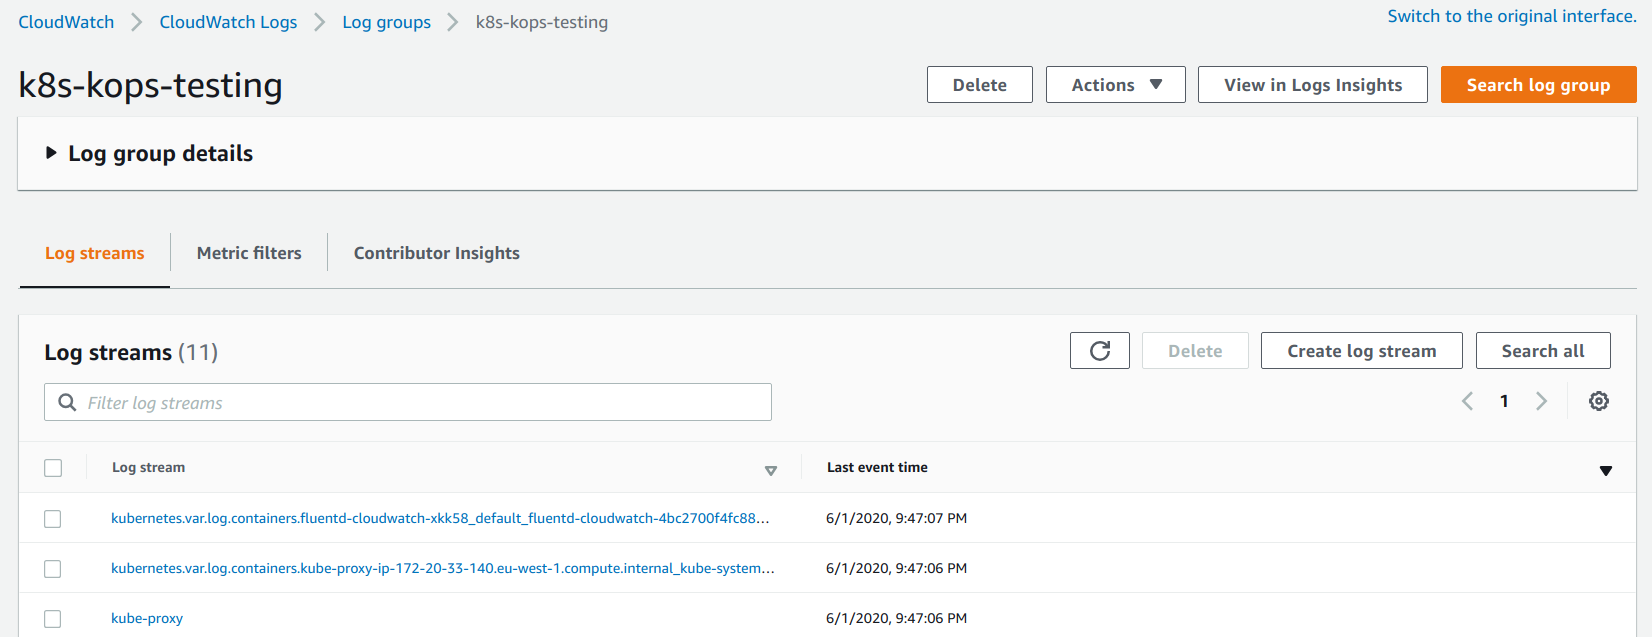
\includegraphics[width=16cm]{figures/kops-testing-cw-logs.png}
    \captionsetup{justification=centering,margin=2cm}
    \caption{AWS CloudWatch with logs from a Kubernetes cluster}}
\end{figure}
\begin{figure}[H]
    \centering
    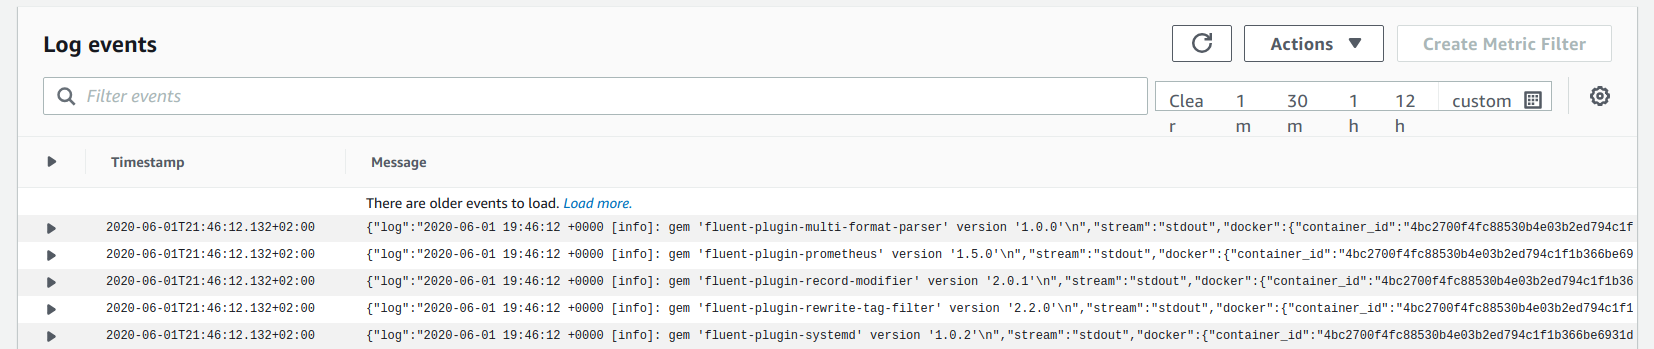
\includegraphics[width=16cm]{figures/kops-testing-cw-logs2.png}
    \captionsetup{justification=centering,margin=2cm}
    \caption{AWS CloudWatch with logs from a Kubernetes cluster}}
\end{figure}

An example log message looks like this:
\begin{lstlisting}[basicstyle=\tiny,caption={An example Kubernetes log message, presented on AWS CloudWatch},captionpos=b,language=Bash,xleftmargin=1cm]
{
    "log": "2020-06-01 19:46:12 +0000 [info]: gem 'fluent-plugin-multi-format-parser' version '1.0.0'\n",
    "stream": "stdout",
    "docker": {
        "container_id": "4bc2700f4fc88530b4e03b2ed794c1f1b366be6931d8500a8ccf21503d2c5b97"
    },
    "kubernetes": {
        "container_name": "fluentd-cloudwatch",
        "namespace_name": "default",
        "pod_name": "fluentd-cloudwatch-xkk58",
        "container_image": "fluent/fluentd-kubernetes-daemonset:v1.7.3-debian-cloudwatch-1.0",
        "container_image_id": "docker-pullable://fluent/fluentd-kubernetes-daemonset@sha256:9b8b2f99ea884853205150364eceaac9fff5ea97fc3300cc0080f48c3eac8b8a",
        "pod_id": "9fc38bd1-ff7b-4d29-9593-15796a7e5f94",
        "host": "ip-172-20-33-140.eu-west-1.compute.internal",
        "labels": {
            "app": "fluentd-cloudwatch",
            "controller-revision-hash": "68f7dc7cc",
            "pod-template-generation": "1",
            "release": "fluentd-cloudwatch"
        },
        "master_url": "https://100.64.0.1:443/api",
        "namespace_id": "4044bfd2-e836-43a1-bda1-71da0e985b9a"
    }
}
\end{lstlisting}

\subsubsection{Testing a cluster}
All the tests can be invoked with a single command:
\begin{lstlisting}[basicstyle=\tiny,caption={TODO},captionpos=b,language=Bash,xleftmargin=1cm]
$ ./kops/tasks _test
\end{lstlisting}

This one command runs the following:
\begin{lstlisting}[basicstyle=\tiny,caption={TODO},captionpos=b,language=Bash,xleftmargin=1cm]
$ kops validate cluster ${K8S_EXP_CLUSTER_NAME} --state "s3://${K8S_EXP_KOPS_S3_BUCKET}"
$ cd tests
$ bats tests.bats
\end{lstlisting}

The \textit{kops validate cluster} command is provided by the kops CLI. It checks that all k8s master and worker nodes are running and have "Ready" status, that all the components are healthy and that all pods in the kube-system namespace are running and healthy\cite{online-kops-valid}. The next command runs the Bats-core tests. They test the version of Kubernetes, number of worker nodes and also they deploy a test Helm chart with Apache Server. All the tests and the deployment (and later deletion) of the Apache Helm chart are automated and intended to be idempotent. Thanks to such a test, it is verified that such a Kubernetes cluster is ready to use for the end users.

The test Apache Server serves a very simple website, which all code is just one index.html file with the following contents:
\begin{lstlisting}[basicstyle=\tiny,caption={TODO},captionpos=b,language=Bash,xleftmargin=1cm]
<html>
<head>
<title>Hello world</title>
</head>
<body>
<p>Welcome to my Master Thesis website!</p>
</body>
</html>
\end{lstlisting}
Thus, there is a test that runs: \textit{curl} command and expects that the output contains "Welcome to my Master Thesis website!". Such a test is possible thanks to an ingress resource provided by the Apache Helm Chart. When this ingress is deployed on a Kubernetes cluster on AWS, an Elastic Load Balancer (ELB) is created. ELB is an AWS resource. The ELB provides us with the endpoint that can be used with \textit{curl}.

\subsubsection{Deleting a cluster}

\subsubsection{Troubleshooting}

\textbf{The first problem} was, that the command responsible for creating a cluster did not wait until the cluster was ready. It returned as soon as the AWS resources were scheduled for creation. This was a problem, because if one wanted to create, test and then delete a Kubernetes cluster in a CI pipeline, then the tests would never work. And the pipeline would always fail. The solution for this problem was already described in the section \ref{kops-creating-the-cluster}.

\textbf{The second problem} was how to configure logging to AWS CloudWatch. The documentation of the Helm chart: kube2iam\cite{kube2iam} provided an example command of how to deploy the chart: \textit{helm install stable/kube2iam --name my-release}. But this resulted in errors, which are presented below, thanks to debugging the kube2iam pod.
\begin{lstlisting}[basicstyle=\tiny,caption={TODO},captionpos=b,language=Bash,xleftmargin=1cm]
$ kubectl get pod
NAME                       READY   STATUS             RESTARTS   AGE
kube2iam-2c8vv             0/1     CrashLoopBackOff   9          17m
$ kubectl logs kube2iam-2c8vv
E0601 10:35:53.142224       1 reflector.go:199] github.com/jtblin/kube2iam/vendor/k8s.io/client-go/tools/cache/reflector.go:94: Failed to list *v1.Pod: pods is forbidden: User "system:serviceaccount:default:default" cannot list resource "pods" in API group "" at the cluster scope
E0601 10:35:53.142621       1 reflector.go:199] github.com/jtblin/kube2iam/vendor/k8s.io/client-go/tools/cache/reflector.go:94: Failed to list *v1.Namespace: namespaces is forbidden: User "system:serviceaccount:default:default" cannot list resource "namespaces" in API group "" at the cluster scope
\end{lstlisting}

These errors went away, when the chart was deployed with additional settings set: \textit{helm upgrade "kube2iam" --namespace="default" --wait --atomic --set rbac.create=true stable/kube2iam}.

\textbf{The third problem} concerned the lack of permissions of the fluentd-cloudwatch pod. It manifested in the following way:
\begin{lstlisting}[basicstyle=\tiny,caption={TODO},captionpos=b,language=Bash,xleftmargin=1cm]
$ kubectl logs fluentd-cloudwatch-xkk58
2020-06-01 11:03:14 +0000 [warn]: #0 [out_cloudwatch_logs_host_logs] failed to flush the buffer. retry_time=8 next_retry_seconds=2020-06-01 11:05:22 +0000 chunk="5a703b5e45c9592f24399f9b73acaf43" error_class=Aws::CloudWatchLogs::Errors::AccessDeniedException error="User: arn:aws:sts::976184668068:assumed-role/nodes.testing.k8s-kops-for-masters-thesis.k8s.local/i-04a926040234f36d6 is not authorized to perform: logs:DescribeLogGroups on resource: arn:aws:logs:eu-west-1:976184668068:log-group::log-stream:"
\end{lstlisting}
This problem was also already dealt with in the section \ref{kops-creating-the-cluster}. The solution was to add IAM permissions in the YAML template configuration file. The solution was inspired by a Tobias Sturm's blog post\cite{kops-logs-cw-tobias} and by the kops documentation\cite{online-kops-iam}.

\textbf{The fourth problem} was with testing the Apache Server. The essential thing to know is that it takes some time (around 5 minutes) for the ELB to be usable by end users and thus the tests may fail in the meantime. The solution was to implement such a command that verifies the Apache Server endpoint many times, but has a maximum number of trials.


* autoscaling from https://learnk8s.io/blog/kubernetes-chaos-engineering-lessons-learned to display the hostname of the current pod in a web page (so that we know if many pods are deployed?); kubectl scale then!

% "Service: A Kubernetes Service that identifies a set of Pods using label selectors. Unless mentioned otherwise, Services are assumed to have virtual IPs only routable within the cluster network." thus we use ingress https://kubernetes.io/docs/concepts/services-networking/ingress/ ; "Kubernetes Service with type: LoadBalancer -> Each Service spawns its own ELB, incurring extra cost." https://medium.com/@dmaas/amazon-eks-ingress-guide-8ec2ec940a70


\begin{lstlisting}[basicstyle=\tiny,caption={TODO},captionpos=b,language=Bash,xleftmargin=1cm]
\end{lstlisting}

labels https://github.com/kubernetes/kops/blob/master/docs/manifests_and_customizing_via_api.md https://github.com/kubernetes/kops/blob/master/docs/labels.md

\subsection{Production deployment using eksctl}
\textit{This section briefly presents all the steps performed that lead to a Kubernetes cluster deployment on the AWS cloud using eksctl. Here an attempt was made to satisfy all the production environment requirements selected in the chapter: \ref{prep-prod}.}
\\

\subsection{TODO}

troubleshooting k8s -mastering k8s p. 58
* what happens if we manually delete a iptables rule? kube-proxy will put it back after 10 to 30s - https://learnk8s.io/blog/kubernetes-chaos-engineering-lessons-learned
* https://learnk8s.io/troubleshooting-deployments - must read!!
